% Options for packages loaded elsewhere
\PassOptionsToPackage{unicode}{hyperref}
\PassOptionsToPackage{hyphens}{url}
%
\documentclass[
  landscape]{article}
\usepackage{lmodern}
\usepackage{amssymb,amsmath}
\usepackage{ifxetex,ifluatex}
\ifnum 0\ifxetex 1\fi\ifluatex 1\fi=0 % if pdftex
  \usepackage[T1]{fontenc}
  \usepackage[utf8]{inputenc}
  \usepackage{textcomp} % provide euro and other symbols
\else % if luatex or xetex
  \usepackage{unicode-math}
  \defaultfontfeatures{Scale=MatchLowercase}
  \defaultfontfeatures[\rmfamily]{Ligatures=TeX,Scale=1}
\fi
% Use upquote if available, for straight quotes in verbatim environments
\IfFileExists{upquote.sty}{\usepackage{upquote}}{}
\IfFileExists{microtype.sty}{% use microtype if available
  \usepackage[]{microtype}
  \UseMicrotypeSet[protrusion]{basicmath} % disable protrusion for tt fonts
}{}
\makeatletter
\@ifundefined{KOMAClassName}{% if non-KOMA class
  \IfFileExists{parskip.sty}{%
    \usepackage{parskip}
  }{% else
    \setlength{\parindent}{0pt}
    \setlength{\parskip}{6pt plus 2pt minus 1pt}}
}{% if KOMA class
  \KOMAoptions{parskip=half}}
\makeatother
\usepackage{xcolor}
\IfFileExists{xurl.sty}{\usepackage{xurl}}{} % add URL line breaks if available
\IfFileExists{bookmark.sty}{\usepackage{bookmark}}{\usepackage{hyperref}}
\hypersetup{
  pdftitle={Statistical Inference: Peer Assessment},
  hidelinks,
  pdfcreator={LaTeX via pandoc}}
\urlstyle{same} % disable monospaced font for URLs
\usepackage[margin=1in]{geometry}
\usepackage{color}
\usepackage{fancyvrb}
\newcommand{\VerbBar}{|}
\newcommand{\VERB}{\Verb[commandchars=\\\{\}]}
\DefineVerbatimEnvironment{Highlighting}{Verbatim}{commandchars=\\\{\}}
% Add ',fontsize=\small' for more characters per line
\usepackage{framed}
\definecolor{shadecolor}{RGB}{248,248,248}
\newenvironment{Shaded}{\begin{snugshade}}{\end{snugshade}}
\newcommand{\AlertTok}[1]{\textcolor[rgb]{0.94,0.16,0.16}{#1}}
\newcommand{\AnnotationTok}[1]{\textcolor[rgb]{0.56,0.35,0.01}{\textbf{\textit{#1}}}}
\newcommand{\AttributeTok}[1]{\textcolor[rgb]{0.77,0.63,0.00}{#1}}
\newcommand{\BaseNTok}[1]{\textcolor[rgb]{0.00,0.00,0.81}{#1}}
\newcommand{\BuiltInTok}[1]{#1}
\newcommand{\CharTok}[1]{\textcolor[rgb]{0.31,0.60,0.02}{#1}}
\newcommand{\CommentTok}[1]{\textcolor[rgb]{0.56,0.35,0.01}{\textit{#1}}}
\newcommand{\CommentVarTok}[1]{\textcolor[rgb]{0.56,0.35,0.01}{\textbf{\textit{#1}}}}
\newcommand{\ConstantTok}[1]{\textcolor[rgb]{0.00,0.00,0.00}{#1}}
\newcommand{\ControlFlowTok}[1]{\textcolor[rgb]{0.13,0.29,0.53}{\textbf{#1}}}
\newcommand{\DataTypeTok}[1]{\textcolor[rgb]{0.13,0.29,0.53}{#1}}
\newcommand{\DecValTok}[1]{\textcolor[rgb]{0.00,0.00,0.81}{#1}}
\newcommand{\DocumentationTok}[1]{\textcolor[rgb]{0.56,0.35,0.01}{\textbf{\textit{#1}}}}
\newcommand{\ErrorTok}[1]{\textcolor[rgb]{0.64,0.00,0.00}{\textbf{#1}}}
\newcommand{\ExtensionTok}[1]{#1}
\newcommand{\FloatTok}[1]{\textcolor[rgb]{0.00,0.00,0.81}{#1}}
\newcommand{\FunctionTok}[1]{\textcolor[rgb]{0.00,0.00,0.00}{#1}}
\newcommand{\ImportTok}[1]{#1}
\newcommand{\InformationTok}[1]{\textcolor[rgb]{0.56,0.35,0.01}{\textbf{\textit{#1}}}}
\newcommand{\KeywordTok}[1]{\textcolor[rgb]{0.13,0.29,0.53}{\textbf{#1}}}
\newcommand{\NormalTok}[1]{#1}
\newcommand{\OperatorTok}[1]{\textcolor[rgb]{0.81,0.36,0.00}{\textbf{#1}}}
\newcommand{\OtherTok}[1]{\textcolor[rgb]{0.56,0.35,0.01}{#1}}
\newcommand{\PreprocessorTok}[1]{\textcolor[rgb]{0.56,0.35,0.01}{\textit{#1}}}
\newcommand{\RegionMarkerTok}[1]{#1}
\newcommand{\SpecialCharTok}[1]{\textcolor[rgb]{0.00,0.00,0.00}{#1}}
\newcommand{\SpecialStringTok}[1]{\textcolor[rgb]{0.31,0.60,0.02}{#1}}
\newcommand{\StringTok}[1]{\textcolor[rgb]{0.31,0.60,0.02}{#1}}
\newcommand{\VariableTok}[1]{\textcolor[rgb]{0.00,0.00,0.00}{#1}}
\newcommand{\VerbatimStringTok}[1]{\textcolor[rgb]{0.31,0.60,0.02}{#1}}
\newcommand{\WarningTok}[1]{\textcolor[rgb]{0.56,0.35,0.01}{\textbf{\textit{#1}}}}
\usepackage{graphicx,grffile}
\makeatletter
\def\maxwidth{\ifdim\Gin@nat@width>\linewidth\linewidth\else\Gin@nat@width\fi}
\def\maxheight{\ifdim\Gin@nat@height>\textheight\textheight\else\Gin@nat@height\fi}
\makeatother
% Scale images if necessary, so that they will not overflow the page
% margins by default, and it is still possible to overwrite the defaults
% using explicit options in \includegraphics[width, height, ...]{}
\setkeys{Gin}{width=\maxwidth,height=\maxheight,keepaspectratio}
% Set default figure placement to htbp
\makeatletter
\def\fps@figure{htbp}
\makeatother
\setlength{\emergencystretch}{3em} % prevent overfull lines
\providecommand{\tightlist}{%
  \setlength{\itemsep}{0pt}\setlength{\parskip}{0pt}}
\setcounter{secnumdepth}{-\maxdimen} % remove section numbering

\title{Statistical Inference: Peer Assessment}
\author{}
\date{\vspace{-2.5em}}

\begin{document}
\maketitle

\hypertarget{part-1-simulation-exercise-instructions}{%
\subsubsection{Part 1: Simulation Exercise
Instructions}\label{part-1-simulation-exercise-instructions}}

Objective: we aimed to investigate the exponential distribution in R and
to compare it with the Central Limit Theorem. We investigated the
distribution of averages of 40 exponentials with a thousand simulations.

We create a dataframe with 1000 means of 40 exponentials.

\begin{Shaded}
\begin{Highlighting}[]
\NormalTok{n <-}\StringTok{ }\DecValTok{40}\NormalTok{; lambda <-}\StringTok{ }\FloatTok{0.2}\NormalTok{; nosim <-}\StringTok{ }\DecValTok{1000}\NormalTok{;}
\CommentTok{# Create a matrix with a size n*nosim  }
\NormalTok{m <-}\StringTok{ }\KeywordTok{matrix}\NormalTok{(}\DataTypeTok{data =} \KeywordTok{rexp}\NormalTok{(nosim }\OperatorTok{*}\StringTok{ }\NormalTok{n, lambda), }\DataTypeTok{nrow =}\NormalTok{ nosim)}
\CommentTok{# Calculate mean of each row}
\NormalTok{df <-}\StringTok{ }\KeywordTok{data.frame}\NormalTok{(}\DataTypeTok{x =} \KeywordTok{apply}\NormalTok{(m, }\DecValTok{1}\NormalTok{, mean))}
\KeywordTok{str}\NormalTok{(df)}
\end{Highlighting}
\end{Shaded}

\begin{verbatim}
## 'data.frame':    1000 obs. of  1 variable:
##  $ x: num  4.81 5.35 4.4 3.31 6.68 ...
\end{verbatim}

\begin{Shaded}
\begin{Highlighting}[]
\KeywordTok{head}\NormalTok{(df)}
\end{Highlighting}
\end{Shaded}

\begin{verbatim}
##          x
## 1 4.812378
## 2 5.350954
## 3 4.402016
## 4 3.309121
## 5 6.675992
## 6 5.687666
\end{verbatim}

We understood the true mean of exponential distribution is 1/lambda and
the standard deviation is also 1/lambda. Then, we can calculate the
theoretical standard deviation,and the theoretical variance, show how
variable the sample is (via variance) and compare it to the theoretical
variance of the distribution.

\begin{Shaded}
\begin{Highlighting}[]
\NormalTok{a <-}\StringTok{ }\KeywordTok{round}\NormalTok{(}\KeywordTok{c}\NormalTok{(}\DataTypeTok{theoretical.mean =} \DecValTok{1}\OperatorTok{/}\NormalTok{lambda, }\DataTypeTok{sample.mean =} \KeywordTok{mean}\NormalTok{(df}\OperatorTok{$}\NormalTok{x), }
             \DataTypeTok{theoretical.sd =}\NormalTok{ (}\DecValTok{1}\OperatorTok{/}\NormalTok{lambda)}\OperatorTok{/}\KeywordTok{sqrt}\NormalTok{(n), }\DataTypeTok{sample.sd =} \KeywordTok{sd}\NormalTok{(df}\OperatorTok{$}\NormalTok{x),}
             \DataTypeTok{theoretical.variance =}\NormalTok{ (}\DecValTok{1}\OperatorTok{/}\NormalTok{lambda)}\OperatorTok{/}\KeywordTok{sqrt}\NormalTok{(n), }\DataTypeTok{sample.variance =}\NormalTok{ ((}\DecValTok{1}\OperatorTok{/}\NormalTok{lambda)}\OperatorTok{/}\KeywordTok{sqrt}\NormalTok{(n))}\OperatorTok{^}\DecValTok{2}\NormalTok{)}
\NormalTok{           ,}\DecValTok{3}\NormalTok{)}
\NormalTok{a}
\end{Highlighting}
\end{Shaded}

\begin{verbatim}
##     theoretical.mean          sample.mean       theoretical.sd 
##                5.000                4.988                0.791 
##            sample.sd theoretical.variance      sample.variance 
##                0.812                0.791                0.625
\end{verbatim}

The results showed that there are a few difference between theoretical
values and sample values.

Finally, we wanted to show that the distribution of averages of 40
exponentials with a thousand simulations is approximately normal.

\begin{Shaded}
\begin{Highlighting}[]
\KeywordTok{require}\NormalTok{(ggplot2)}
\NormalTok{g <-}\StringTok{ }\KeywordTok{ggplot}\NormalTok{(}\DataTypeTok{data =}\NormalTok{ df, }\KeywordTok{aes}\NormalTok{(}\DataTypeTok{x =}\NormalTok{ x)) }
\NormalTok{g <-}\StringTok{ }\NormalTok{g }\OperatorTok{+}\StringTok{ }\KeywordTok{geom_histogram}\NormalTok{(}\KeywordTok{aes}\NormalTok{(}\DataTypeTok{y =}\NormalTok{ ..density..), }\DataTypeTok{fill =} \StringTok{"lightblue"}\NormalTok{, }\DataTypeTok{binwidth=}\FloatTok{0.2}\NormalTok{, }\DataTypeTok{colour =} \StringTok{"black"}\NormalTok{)}
\NormalTok{g <-}\StringTok{ }\NormalTok{g }\OperatorTok{+}\StringTok{ }\KeywordTok{geom_density}\NormalTok{(}\DataTypeTok{size =} \DecValTok{1}\NormalTok{, }\DataTypeTok{colour =} \StringTok{"black"}\NormalTok{)}
\NormalTok{g}
\end{Highlighting}
\end{Shaded}

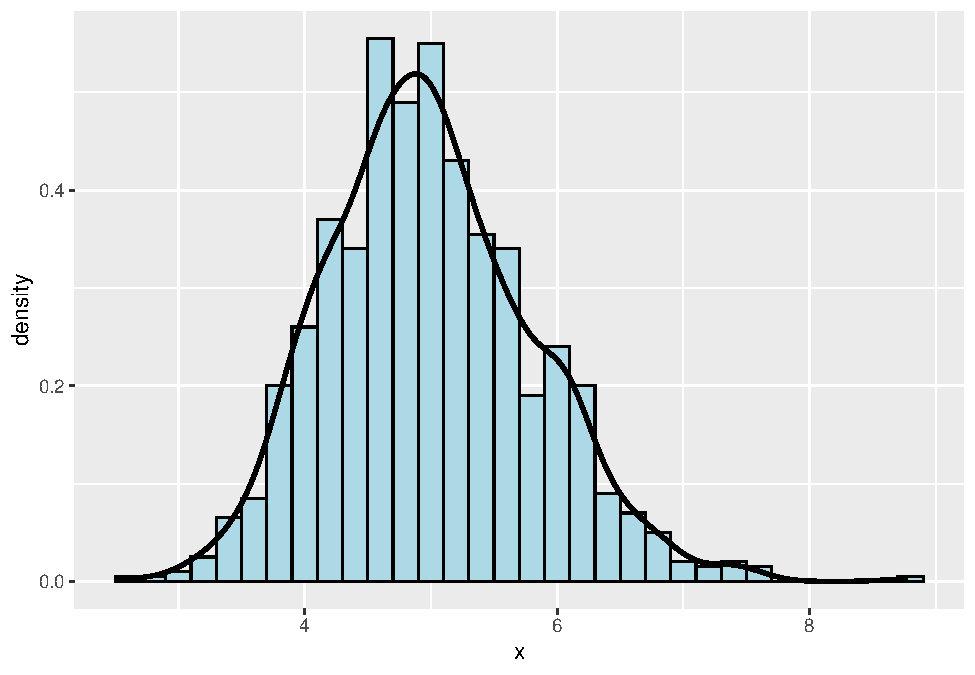
\includegraphics{PA1_files/figure-latex/unnamed-chunk-3-1.pdf}

\hypertarget{part-2-basic-inferential-data-analysis-instructions}{%
\subsubsection{Part 2: Basic Inferential Data Analysis
Instructions}\label{part-2-basic-inferential-data-analysis-instructions}}

Objective:

\hypertarget{load-the-toothgrowth-data-and-perform-some-basic-exploratory-data-analyses.}{%
\paragraph{2.1 Load the ToothGrowth data and perform some basic
exploratory data
analyses.}\label{load-the-toothgrowth-data-and-perform-some-basic-exploratory-data-analyses.}}

According to the package description, the data is about the length of
odontoblasts (cells responsible for tooth growth) in 60 guinea pigs.
Each animal received one of three dose levels of vitamin C (0.5, 1, and
2 mg/day) by one of two delivery methods, orange juice or ascorbic acid
(a form of vitamin C and coded as VC).

The data contain a data frame with 60 observations on 3 variables.

\begin{enumerate}
\def\labelenumi{\arabic{enumi}.}
\tightlist
\item
  {[}len{]} numeric Tooth length
\item
  {[}supp{]} factor Supplement type (VC or OJ).
\item
  {[}dose{]} numeric Dose in milligrams/day:
\end{enumerate}

\begin{Shaded}
\begin{Highlighting}[]
\CommentTok{# Load data}
\KeywordTok{library}\NormalTok{(datasets)}
\KeywordTok{data}\NormalTok{(ToothGrowth)}

\CommentTok{# Preview data}
\KeywordTok{head}\NormalTok{(ToothGrowth, }\DataTypeTok{n =} \DecValTok{5}\NormalTok{)}
\end{Highlighting}
\end{Shaded}

\begin{verbatim}
##    len supp dose
## 1  4.2   VC  0.5
## 2 11.5   VC  0.5
## 3  7.3   VC  0.5
## 4  5.8   VC  0.5
## 5  6.4   VC  0.5
\end{verbatim}

\begin{Shaded}
\begin{Highlighting}[]
\CommentTok{# Preview data by a scatterplot}
\KeywordTok{library}\NormalTok{(ggplot2)}

\NormalTok{g1 <-}\StringTok{ }\KeywordTok{ggplot}\NormalTok{(ToothGrowth, }\KeywordTok{aes}\NormalTok{(}\DataTypeTok{x=}\NormalTok{dose, }\DataTypeTok{y=}\NormalTok{len, }\DataTypeTok{shape=}\NormalTok{supp, }\DataTypeTok{color=}\NormalTok{supp, }\DataTypeTok{size=}\NormalTok{supp)) }\OperatorTok{+}
\StringTok{    }\KeywordTok{geom_point}\NormalTok{(}\DataTypeTok{size=}\DecValTok{2}\NormalTok{, }\DataTypeTok{shape=}\DecValTok{19}\NormalTok{) }\OperatorTok{+}
\StringTok{    }\KeywordTok{labs}\NormalTok{(}\DataTypeTok{x =} \StringTok{"Dose in milligrams/day"}\NormalTok{,}
         \DataTypeTok{y =} \StringTok{"Tooth length"}\NormalTok{,}
         \DataTypeTok{caption =} \StringTok{''}\NormalTok{) }\OperatorTok{+}\StringTok{ }
\StringTok{    }\KeywordTok{ggtitle}\NormalTok{(}\StringTok{"The Effect of Vitamin C on }
\StringTok{Tooth Growth in Guinea Pigs"}\NormalTok{) }\OperatorTok{+}
\StringTok{    }\KeywordTok{labs}\NormalTok{(}\DataTypeTok{color=}\StringTok{"Supplement}
\StringTok{type"}\NormalTok{) }

\CommentTok{# Preview data by a boxplot}
\NormalTok{g2 <-}\StringTok{ }\KeywordTok{ggplot}\NormalTok{(ToothGrowth, }\KeywordTok{aes}\NormalTok{(}\DataTypeTok{x =} \KeywordTok{factor}\NormalTok{(dose), }\DataTypeTok{y =}\NormalTok{ len, }\DataTypeTok{fill =}\NormalTok{ supp)) }\OperatorTok{+}
\StringTok{    }\KeywordTok{geom_boxplot}\NormalTok{() }\OperatorTok{+}
\StringTok{    }\KeywordTok{facet_grid}\NormalTok{(.}\OperatorTok{~}\NormalTok{supp) }\OperatorTok{+}
\StringTok{    }\KeywordTok{ggtitle}\NormalTok{(}\StringTok{"The Effect of Vitamin C on }
\StringTok{Tooth Growth in Guinea Pigs"}\NormalTok{) }\OperatorTok{+}
\StringTok{    }\KeywordTok{scale_x_discrete}\NormalTok{(}\StringTok{"Dose in milligrams/day"}\NormalTok{) }\OperatorTok{+}\StringTok{   }
\StringTok{    }\KeywordTok{scale_y_continuous}\NormalTok{(}\StringTok{"Tooth Length"}\NormalTok{) }\OperatorTok{+}\StringTok{  }
\StringTok{    }\KeywordTok{scale_fill_discrete}\NormalTok{(}\DataTypeTok{name=}\StringTok{"Supplement}
\StringTok{type"}\NormalTok{) }
\KeywordTok{require}\NormalTok{(gridExtra)}
\KeywordTok{grid.arrange}\NormalTok{(g1, g2, }\DataTypeTok{ncol=}\DecValTok{2}\NormalTok{)}
\end{Highlighting}
\end{Shaded}

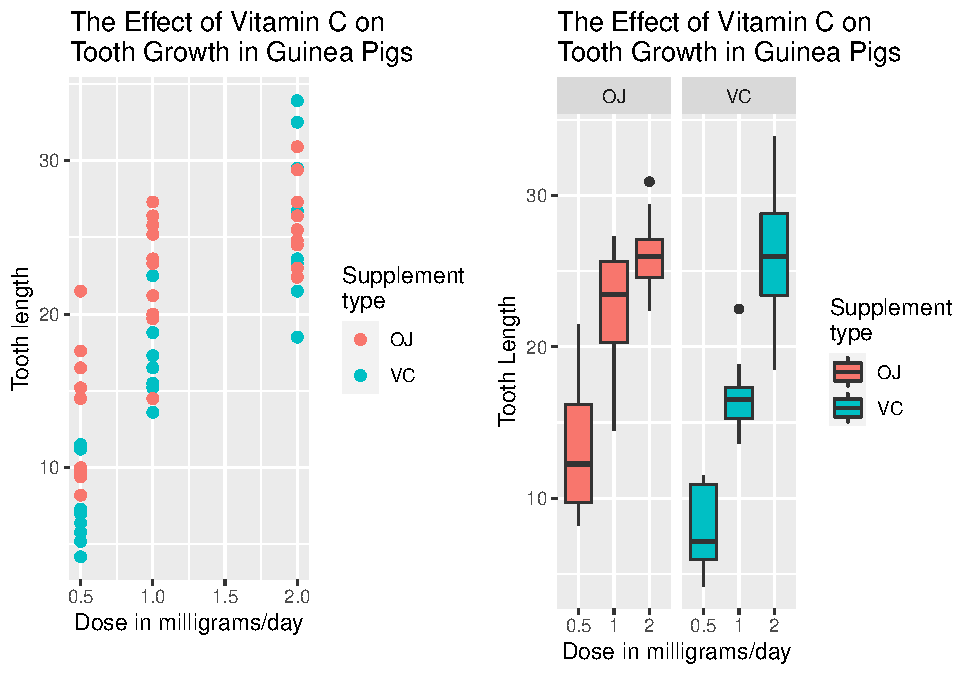
\includegraphics{PA1_files/figure-latex/unnamed-chunk-4-1.pdf}

\hypertarget{provide-a-basic-summary-of-the-data.}{%
\paragraph{2.2 Provide a basic summary of the
data.}\label{provide-a-basic-summary-of-the-data.}}

\begin{Shaded}
\begin{Highlighting}[]
\CommentTok{# Preview any missing values}
\KeywordTok{any}\NormalTok{ (}\KeywordTok{is.na}\NormalTok{(ToothGrowth))}
\end{Highlighting}
\end{Shaded}

\begin{verbatim}
## [1] FALSE
\end{verbatim}

\begin{Shaded}
\begin{Highlighting}[]
\CommentTok{# Preview the dimension}
\KeywordTok{dim}\NormalTok{(ToothGrowth)}
\end{Highlighting}
\end{Shaded}

\begin{verbatim}
## [1] 60  3
\end{verbatim}

\begin{Shaded}
\begin{Highlighting}[]
\CommentTok{# Preview an internal structure}
\KeywordTok{str}\NormalTok{(ToothGrowth)}
\end{Highlighting}
\end{Shaded}

\begin{verbatim}
## 'data.frame':    60 obs. of  3 variables:
##  $ len : num  4.2 11.5 7.3 5.8 6.4 10 11.2 11.2 5.2 7 ...
##  $ supp: Factor w/ 2 levels "OJ","VC": 2 2 2 2 2 2 2 2 2 2 ...
##  $ dose: num  0.5 0.5 0.5 0.5 0.5 0.5 0.5 0.5 0.5 0.5 ...
\end{verbatim}

\begin{Shaded}
\begin{Highlighting}[]
\CommentTok{# Preview a Five-number summary}
\KeywordTok{summary}\NormalTok{(ToothGrowth)}
\end{Highlighting}
\end{Shaded}

\begin{verbatim}
##       len        supp         dose      
##  Min.   : 4.20   OJ:30   Min.   :0.500  
##  1st Qu.:13.07   VC:30   1st Qu.:0.500  
##  Median :19.25           Median :1.000  
##  Mean   :18.81           Mean   :1.167  
##  3rd Qu.:25.27           3rd Qu.:2.000  
##  Max.   :33.90           Max.   :2.000
\end{verbatim}

\begin{Shaded}
\begin{Highlighting}[]
\CommentTok{# Preview data in terms of table}
\KeywordTok{table}\NormalTok{(ToothGrowth}\OperatorTok{$}\NormalTok{supp,ToothGrowth}\OperatorTok{$}\NormalTok{dose, }\DataTypeTok{useNA=}\StringTok{"ifany"}\NormalTok{)}
\end{Highlighting}
\end{Shaded}

\begin{verbatim}
##     
##      0.5  1  2
##   OJ  10 10 10
##   VC  10 10 10
\end{verbatim}

\hypertarget{use-confidence-intervals-andor-hypothesis-tests-to-compare-tooth-growth-by-supp-and-dose.-only-use-the-techniques-from-class-even-if-theres-other-approaches-worth-considering}{%
\paragraph{2.3 Use confidence intervals and/or hypothesis tests to
compare tooth growth by supp and dose. (Only use the techniques from
class, even if there's other approaches worth
considering)}\label{use-confidence-intervals-andor-hypothesis-tests-to-compare-tooth-growth-by-supp-and-dose.-only-use-the-techniques-from-class-even-if-theres-other-approaches-worth-considering}}

Since the sample size for each groups (OJ, VC) is small (n≤30) and
population standard deviation is unknown, the T confidence interval is
used.

\textbf{Question: Is there a statistical difference in the tooth growth
by different delievery method?}

H0:𝜇1−𝜇2 = 0 (there is no difference between the means of two groups
(OJ, VC) in terms of tooth growth) Ha:𝜇1−𝜇2 \textgreater{} 0 (there is a
significant difference between the means of two groups (OJ, VC) in terms
of tooth growth)

Degree of significance, α\% = 5\%; level of significance α = 0.05

To compute the value of test statistic:

\begin{Shaded}
\begin{Highlighting}[]
\CommentTok{# Code: the independent t test with variance equal or unequal assumptions.}
\NormalTok{equal_t <-}\StringTok{ }\KeywordTok{t.test}\NormalTok{(len}\OperatorTok{~}\NormalTok{supp, }\DataTypeTok{paired =} \OtherTok{FALSE}\NormalTok{, }\DataTypeTok{var.equal =} \OtherTok{TRUE}\NormalTok{, }\DataTypeTok{alt =} \StringTok{"greater"}\NormalTok{, }\DataTypeTok{data =}\NormalTok{ ToothGrowth, }\DataTypeTok{conf.level =} \FloatTok{0.95}\NormalTok{)}
\NormalTok{unequal_t <-}\StringTok{ }\KeywordTok{t.test}\NormalTok{(len}\OperatorTok{~}\NormalTok{supp, }\DataTypeTok{paired =} \OtherTok{FALSE}\NormalTok{, }\DataTypeTok{var.equal =} \OtherTok{FALSE}\NormalTok{, }\DataTypeTok{alt =} \StringTok{"greater"}\NormalTok{, }\DataTypeTok{data =}\NormalTok{ ToothGrowth, }\DataTypeTok{conf.level =} \FloatTok{0.95}\NormalTok{)}


\CommentTok{# Code: Permutation tests to test the null hypothesis of no difference between treatment groups.}

\NormalTok{permuatation <-}\StringTok{ }\ControlFlowTok{function}\NormalTok{(y, group, g1_name, g2_name) \{}
    \CommentTok{# to calculate the mean of two groups, notice here group is a variable. }
\NormalTok{    testStat <-}\StringTok{ }\ControlFlowTok{function}\NormalTok{(w, g) }\KeywordTok{mean}\NormalTok{(w[g }\OperatorTok{==}\StringTok{ }\NormalTok{g1_name]) }\OperatorTok{-}\StringTok{ }\KeywordTok{mean}\NormalTok{(w[g }\OperatorTok{==}\StringTok{ }\NormalTok{g2_name])}
    \CommentTok{# To calculate the difference of mean between group OJ and VC. }
\NormalTok{    observedStat <-}\StringTok{ }\KeywordTok{testStat}\NormalTok{(y, group)}
    \CommentTok{#Permutation: change the group label of subdata randomly for 10000 times, i.e., if the group if irrevelant to the y. }
\NormalTok{    permutations <-}\StringTok{ }\KeywordTok{sapply}\NormalTok{(}\DecValTok{1} \OperatorTok{:}\StringTok{ }\DecValTok{10000}\NormalTok{, }\ControlFlowTok{function}\NormalTok{(i) }\KeywordTok{testStat}\NormalTok{(y, }\KeywordTok{sample}\NormalTok{(group)))}
\NormalTok{    permutate_t <-}\StringTok{ }\KeywordTok{sum}\NormalTok{(permutations }\OperatorTok{>}\StringTok{ }\NormalTok{observedStat)}\OperatorTok{/}\DecValTok{10000}
\NormalTok{    permutate_t}
\NormalTok{\}}
\NormalTok{permutate_t <-}\StringTok{ }\KeywordTok{permuatation}\NormalTok{(ToothGrowth}\OperatorTok{$}\NormalTok{len, }\KeywordTok{as.character}\NormalTok{(ToothGrowth}\OperatorTok{$}\NormalTok{supp), }\StringTok{"OJ"}\NormalTok{,}\StringTok{"VC"}\NormalTok{)}

\NormalTok{result <-}\StringTok{ }\KeywordTok{data.frame}\NormalTok{(}
    \StringTok{"p-value"}\NormalTok{ =}\StringTok{ }\KeywordTok{c}\NormalTok{(equal_t}\OperatorTok{$}\NormalTok{p.value, unequal_t}\OperatorTok{$}\NormalTok{p.value, permutate_t),}
    \StringTok{"t statistic"}\NormalTok{ =}\KeywordTok{c}\NormalTok{(equal_t}\OperatorTok{$}\NormalTok{statistic, unequal_t}\OperatorTok{$}\NormalTok{statistic, }\StringTok{""}\NormalTok{)}
\NormalTok{)}
\KeywordTok{row.names}\NormalTok{(result) <-}\StringTok{ }\KeywordTok{c}\NormalTok{(}\StringTok{"var.equal"}\NormalTok{, }\StringTok{"var.unequal"}\NormalTok{, }\StringTok{"permutation test"}\NormalTok{)}
\NormalTok{result}
\end{Highlighting}
\end{Shaded}

\begin{verbatim}
##                     p.value      t.statistic
## var.equal        0.03019669 1.91526826869527
## var.unequal      0.03031725 1.91526826869527
## permutation test 0.03170000
\end{verbatim}

\textbf{Answer}: Since all p-values less than 0.05 were statistically
significant, it indicated strong evidence against the null hypothesis
(no difference between then length and the methods of delivery). There
were less than a 5\% probability the null is correct (and the results
are random). Therefore, we rejected the null hypothesis, and accepted
the alternative hypothesis.

\textbf{Sub-question}: Different levels of dose by VC or OJ might bring
different impacts on the tooth length. So, we continued to investigate
them.

\textbf{Answer}: Because of the big intra-group variance, the unpaired t
test gave a confidence interval containing 0. So we could not rule out
that the two group are different.

As a result, there was a difference in the tooth growth by different
delivery methods (VC versus OJ) of .5 and 1 milligrams/day, since the
unpaired t test did not a confidence interval containing 0.

However for the delivery method of 2 milligrams/day, at 𝛼= 0.05, we
cannot conclude a significant difference (VC versus OJ) between 𝜇1 and
𝜇2 if the 95\% confidence interval contains 0. VC and OJ both could
provide a very similar result.

\hypertarget{state-your-conclusions-and-the-assumptions-needed-for-your-conclusions.}{%
\paragraph{2.4 State your conclusions and the assumptions needed for
your
conclusions.}\label{state-your-conclusions-and-the-assumptions-needed-for-your-conclusions.}}

\end{document}
